\documentclass[tikz,border=2pt]{standalone}
\usepackage{amsmath,amssymb}
\usepackage{tikz}
\usetikzlibrary{arrows.meta}

\begin{document}
% With objective 2 x_s + 2 x_t the objective lines are parallel to the edge x_s + x_t = 80:
% every point of that edge, from (0,80) to (20,60), is optimal with z = 160.
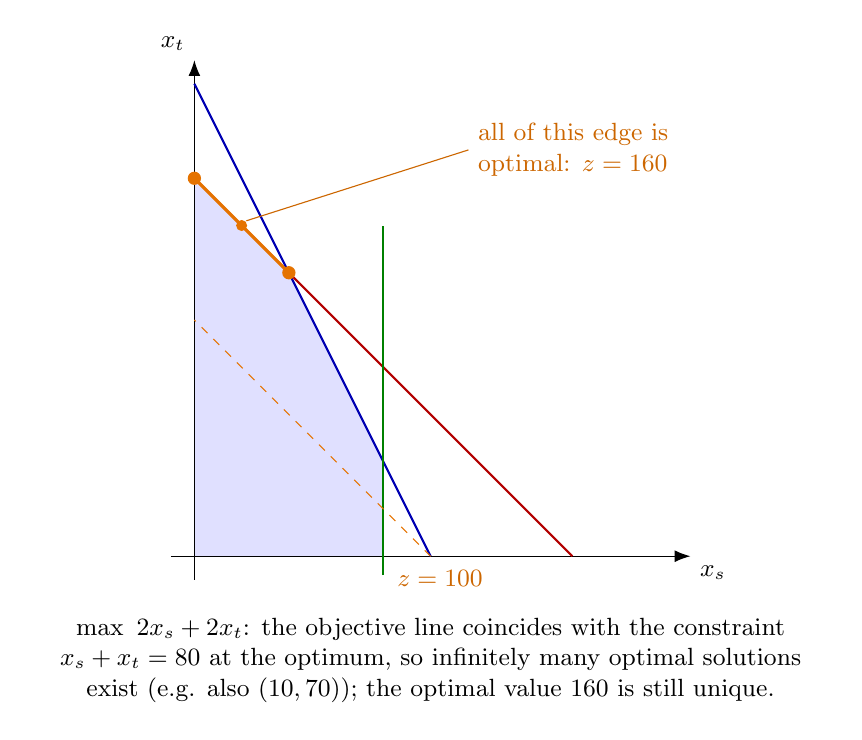
\begin{tikzpicture}[x=0.06cm, y=0.06cm, every node/.style={font=\small}, >={Latex[length=2mm]}]
	\fill[blue!12] (0,0) -- (40,0) -- (40,20) -- (20,60) -- (0,80) -- cycle;
	\draw[->] (-5,0) -- (105,0) node[below right] {$x_s$};
	\draw[->] (0,-5) -- (0,105) node[above left] {$x_t$};
	\draw[blue!70!black, thick] (50,0) -- (0,100);
	\draw[red!70!black, thick] (80,0) -- (0,80);
	\draw[green!50!black, thick] (40,-4) -- (40,70);
	\draw[orange!90!black, dashed] (50,0) -- (0,50);
	\node[orange!80!black, anchor=north] at (52,-1) {$z=100$};
	\draw[orange!90!black, very thick] (0,80) -- (20,60);
	\fill[orange!90!black] (0,80) circle (2.4pt);
	\fill[orange!90!black] (20,60) circle (2.4pt);
	\fill[orange!90!black] (10,70) circle (2pt);
	\draw[orange!80!black, thin] (11,71) -- (58,86);
	\node[orange!80!black, anchor=west, align=left] at (58,86) {all of this edge is\\ optimal: $z=160$};
	\node[anchor=north, align=flush center, text width=10cm] at (50,-11) {$\max\ 2x_s+2x_t$: the objective line coincides with the constraint $x_s+x_t=80$ at the optimum, so infinitely many optimal solutions exist (e.g. also $(10,70)$); the optimal value $160$ is still unique.};
\end{tikzpicture}
\end{document}
